\documentclass[10pt]{beamer}

\usepackage[utf8]{inputenc}
\usepackage{tcolorbox}
\usepackage{tikz}
\usepackage{tikz-3dplot}
\usetikzlibrary{intersections,calc,,angles,quotes,through}
\usepackage{amsmath}
\usepackage{graphicx}
\usepackage{cases}
\def \heart {\textcolor{blue}{$\heartsuit$} }
\def \C {\mathcal{C}}
\def \orthog {\underline{\perp}}
\def\arcos{\operatorname{arcos}}
\def \deg {^{\circ}}

\newcommand{\vect}[1] {
  \overrightarrow{#1}}

\tcbset{%
	basic/.style={colframe=black,
		      colback=white,
		      top= 0mm,
		      bottom = 2mm,
		      boxsep=0mm
		      }
}
\tikzset{
    invisible/.style={opacity=0},
    visible on/.style={alt={#1{}{invisible}}},
    alt/.code args={<#1>#2#3}{%
      \alt<#1>{\pgfkeysalso{#2}}{\pgfkeysalso{#3}} % \pgfkeysalso doesn't change the path
    },
  }

    
\begin{document}  
    \beamertemplatenavigationsymbolsempty
    \setlength{\abovedisplayskip}{0pt}
    \setlength{\belowdisplayskip}{0pt}
    \frame{
	  
	  \frametitle{Q3 Juillet 2004.}
	  %\renewcommand{\theenumi}{\alph{enumi})}
	  Soit $ABC$ un triangle tel que l’angle $\widehat{A}$ soit obtus. On note $E$ la projection
	  orthogonale de $B$ sur $AC$ et $F$ la projection orthogonale de $C$ sur $AB$. \\ \smallskip
	  Démontrer que $|\vect{BC}|^2 = |\vect{AB}||\vect{BF}| + |\vect{AC}||\vect{CE}|$.  
	  \vfill
	  
	  \pause
	  % hypothèses et thèse
	  \begin{tcolorbox}[basic] 
	      \begin{columns}[t]
		 
		 \column{.5\textwidth}\centering
		      
		      \underline{Hypothèses} 
		      \begin{itemize}
		      \item $BE \bot AC$,
		      \item $CF \bot AB$.
		      \end{itemize}

		  
		  \column{.5\textwidth}\centering
		      
		      \underline{Thèse} \\
		      \smallskip
		      $|\vect{BC}|^2 = |\vect{AB}||\vect{BF}| + |\vect{AC}||\vect{CE}|$.  
		
	      \end{columns}
	  \end{tcolorbox}
    }

    \frame{ 
	  % résolution ex1
	  \begin{columns}[t]
		\column{.5\textwidth}\centering 
		

			\underline{Dessin}\\
			
				  \begin{figure}[h]
				  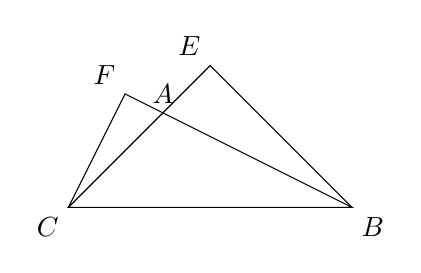
\begin{tikzpicture}[scale=0.8]
			          %projection ($(X)!(B')!(B)$)
			          %nommer chemin 'name path
			          %intersection \path [name intersections={of=d and gb,name=G}];
			          %animation  \draw[visible on=<1>] 
				  %           \draw[visible on=<{2,4}>]
				  %angle arc[radius = 6mm, start angle= 180, end angle= 225] node [below left,pos=0.3]{$\alpha$}
				  %angle \pic [draw,"$\alpha$", angle eccentricity=1.5] {angle = A'--A--B};
				  %perpendiculaire ($(A')!3cm!-90:(A)$)
				  %cercle par point \node [draw] at (A) [circle through=(B)] {};
				  
				   %TRIANGLE ABC
				  \coordinate[label=below left:$C$] (C) at (-1.5,0);
				  \coordinate[label=below right:$B$] (B) at (3,0);
				  \coordinate[label=above:$A$] (A) at (0,1.5);
				  \draw (A) -- (B) -- (C) -- cycle;		
				  
				  %E,F
				  \draw [name path=BE] (B) -- ($(A)!(B)!(C)$) coordinate[label=above left:$E$] (E) -- (A);
				  \draw [name path=CF] (C) -- ($(A)!(C)!(B)$) coordinate[label=above left:$F$] (F) -- (A);
				  \end{tikzpicture}
				  \end{figure}
			
				  \begin{tcolorbox}[basic] 
				      
				    \smallskip
				    \underline{Hypothèses} 
				    \begin{enumerate}
				     \item $BE \bot AC$,
				     \item $CF \bot AB$.  
				    \end{enumerate}
							      
				    \underline{Thèse} \\
				    \smallskip
				    $|\vect{BC}|^2 = |\vect{AB}||\vect{BF}| + |\vect{AC}||\vect{CE}|$.  
				    \end{tcolorbox}
		
		
		\column{.5\textwidth}\centering
		
		\underline{Résolution}\\ \flushleft
		
		\heart Le produit scalaire de 2 vecteurs perpendiculaires est nul.\\
		
		\begin{align*}
		 &|\vect{AB}||\vect{BF}| + |\vect{AC}||\vect{CE}| \\
		 = \ & |\vect{BA}||\vect{BF}| + |\vect{CA}||\vect{CE}|, \\
		 = \ & \vect{BA}\cdot\vect{BF} + \vect{CA}\cdot\vect{CE}, \text{ (points alignés)} \\
		 = \ & \vect{BA}\cdot(\vect{BF} + \vect{FC}) + \vect{CA}\cdot(\vect{CE}+\vect{EB}), \text{ (\textcolor{blue}{1} et \textcolor{blue}{2})} \\
		 = \ & \vect{BA}\cdot\vect{BC} + \vect{CA}\cdot\vect{CB}, \\
		 = \ & \vect{BC}\cdot(\vect{BA} - \vect{CA}), \\
		 = \ & \vect{BC}\cdot\vect{BC} = |\vect{BC}|^2.
		\end{align*} \\
		\hfill $\qed$
		
		%\centering\noindent\rule{2cm}{0.4pt}
	        %\hfill $\qed$

   
	   \end{columns}
    
    
    
    }
	  
  
\end{document}
